\documentclass{beamer}
\usepackage[english]{babel}
\usepackage[round]{natbib}
\usepackage{color}

% ============================
%  Figures and relative paths
% ============================
\usepackage{graphicx}
\graphicspath{{figures/}}

% =================
%  Beamer options
% =================
\usetheme{default}
\setbeamertemplate{footline}[frame number]
\usecolortheme{rose}

\setbeamerfont{section title}{parent=title}
\setbeamercolor{section title}{parent=titlelike}
%\defbeamertemplate*{section page}{default}[1][]
%{
  %\centering
    %\begin{beamercolorbox}[sep=8pt,center,#1]{section title}
%      \usebeamerfont{section title}\insertsection\par
%    \end{beamercolorbox}
%}
%\newcommand*{\sectionpage}{\usebeamertemplate*{section page}}


% ==========
%  Document
% ==========
\begin{document}

\title{\texttt{rba} Python package}
\date{24/10/2017}
\maketitle

\begin{frame}{Resource Allocation}
  \begin{figure}[!ht]
    \centering
    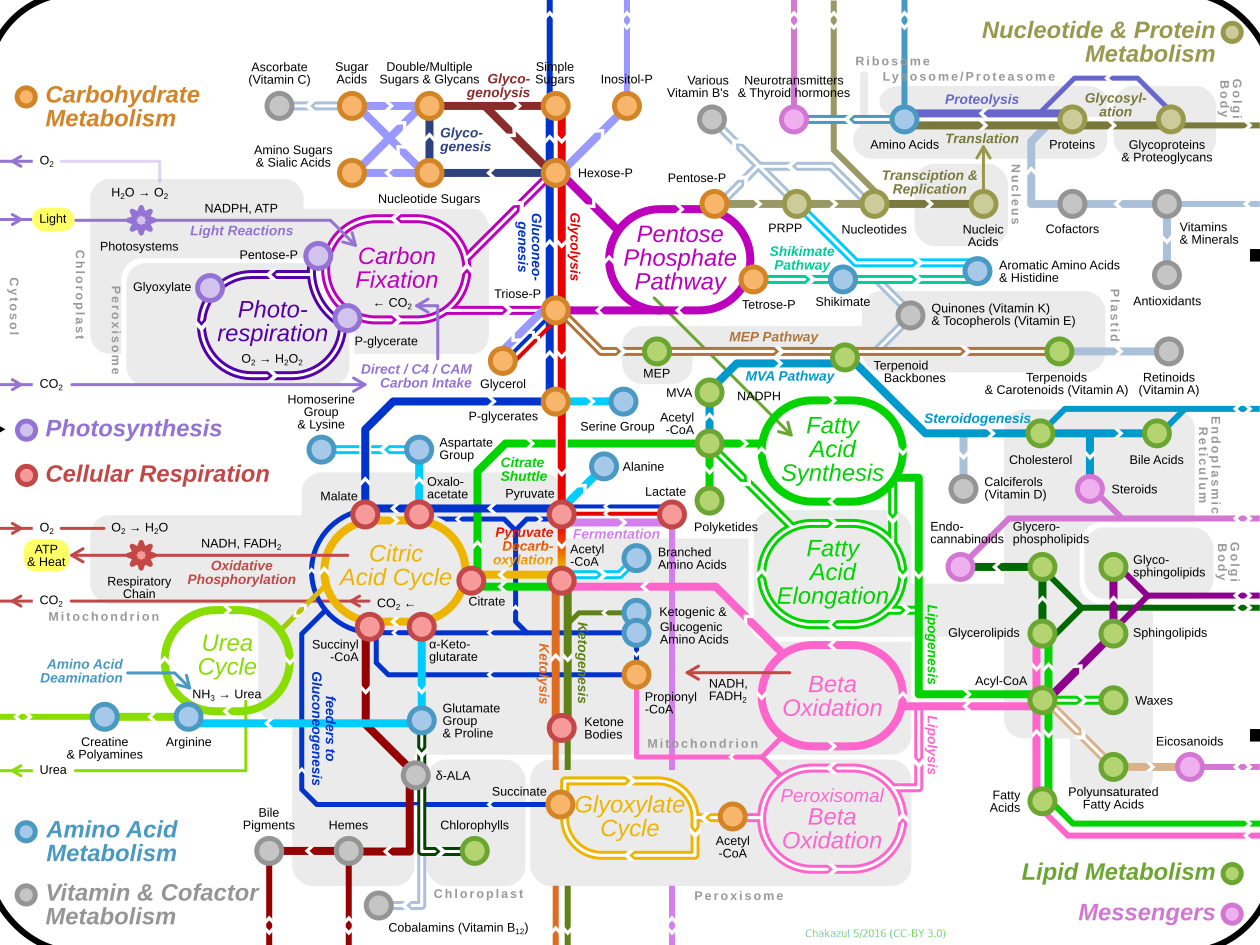
\includegraphics[width=\linewidth]{intro}
  \end{figure}
\end{frame}

\begin{frame}{RBA constraints}
  Resource Balance Analysis (RBA) implements 3 sets of constraints.
  \begin{itemize}
    \item \textbf{Mass conservation}: chemical reactions
    (metabolic reaction, protein synthesis)
    and boundary conditions (import/export, creation of biomass).

    $\rightarrow$ basic Flux Balance Analysis constraint.

    \item \textbf{Capacity constraints}: a reaction flux can only be sustained
    if there are enough enzymes (or ribosomes, chaperones).

    $\rightarrow$ sets a price for every metabolic pathway.

    \item \textbf{Maximal density}: every compartment holds a limited number
    of molecular species.

    $\rightarrow$ selection of most parsimonious pathways.
  \end{itemize}
\end{frame}

\begin{frame}{rba package}
  \textbf{Objective}: adapt rba algorithm to any organism.
  \begin{figure}[!ht]
    \centering
    \includegraphics[width=0.8\linewidth]{package_structure}
  \end{figure}
\end{frame}

\begin{frame}{rba.xml}
  \textbf{Principles}
  \begin{itemize}
    \item Explicit all requirements for an RBA model.
    \item Regroup related pieces of information (modular structure).
  \end{itemize}
\end{frame}

\begin{frame}[fragile]{rba.xml mirrors the structure of XML files}
  \begin{figure}[!ht]
    \centering
    \includegraphics[width=\linewidth]{xml_python_mirror}
  \end{figure}
\end{frame}

\begin{frame}{RBA models are composed of 8 files}
  \begin{figure}[!ht]
    \centering
    \includegraphics[width=\linewidth]{xml_files}
  \end{figure}
\end{frame}

\begin{frame}{Information related to mass conservation}
  \begin{figure}[!ht]
    \centering
    \includegraphics[width=\linewidth]{xml_mass_conservation}
  \end{figure}
\end{frame}

\begin{frame}{Information related to machinery capacities}
  \begin{figure}[!ht]
    \centering
    \includegraphics[width=\linewidth]{xml_capacity_constraints}
  \end{figure}
\end{frame}

\begin{frame}{Information related to density}
  \begin{figure}[!ht]
    \centering
    \includegraphics[width=\linewidth]{xml_density_constraints}
  \end{figure}
\end{frame}

\begin{frame}{Differences with SBML standard}
  \begin{itemize}
    \item Modularity: no need to regenerate everything if you just want
    to change the external medium.
    \item Growth rate dependent functions.
    \item Targets can be concentrations.
  \end{itemize}
\end{frame}

\begin{frame}{rba.prerba}
  \textbf{Principles}
  \begin{itemize}
    \item Generate minimal RBA model from existing SBML model.
    \item Retrieve missing information automatically. Ask user to contribute
    only when necessary.
    \item Generate only valid models (that can be solved).
  \end{itemize}
\end{frame}

\begin{frame}{rba.prerba flow}
  \begin{figure}[!ht]
    \centering
    \includegraphics[width=\linewidth]{prerba_summary}
  \end{figure}
  The RBA model uses default values where necessary.
  The user can provide more accurate values by communicating through
  helper files.
\end{frame}

\begin{frame}{rba.prerba example (1)}
  \begin{figure}[!ht]
    \centering
    \includegraphics[width=0.8\linewidth]{example_1}

    \includegraphics[width=0.8\linewidth]{example_2}
  \end{figure}
\end{frame}

\begin{frame}{rba.prerba example (2)}
  \begin{figure}[!ht]
    \centering
    \includegraphics[width=0.8\linewidth]{example_3}

    \includegraphics[width=0.8\linewidth]{example_4}
  \end{figure}
\end{frame}

\begin{frame}{rba.prerba helper file example}
  \begin{figure}[!ht]
    \centering
    \includegraphics[width=\linewidth]{subunits_example}
  \end{figure}
\end{frame}

\begin{frame}{rba.prerba helper files}
  \begin{itemize}
    \item unknown\_proteins.tsv: SBML gene identifier not found in uniprot.
    \item cofactors.tsv: ambiguous protein cofactors.
    \item subunits.tsv: ambiguous/missing protein stoichiometry.
    \item locations.tsv: ambiguous/missing protein location.
    \item location\_mapping.tsv: by default, uniprot compartment are used.
    User may change compartment identifiers here.
    \item metabolites.tsv: biomass production, key metabolites
    (cofactors, metabolites needed in protein synthesis) not retrieved in SBML.\@
    \item macrocomponents.tsv: biomass production targets.
    \item fasta files with default composition of tRNAs, ribosomes and
    chaperones.
  \end{itemize}
\end{frame}

\begin{frame}{rba.prerba usage}
  \begin{itemize}
    \item Generate a first model, solve it.
    \item Fill in information in helper files, generate a fully functional
    model.
    \item Adapt enzyme efficiencies using rba.xml.
    \item Add new processes using rba.xml.
  \end{itemize}
\end{frame}

\begin{frame}{rba.core}
  \textbf{Principles}
  \begin{itemize}
    \item Remove any hard-coded information.
    \item Convert model into matrix blocks that can be rearranged during
    solving.
  \end{itemize}
\end{frame}

\begin{frame}{rba.core idea}
  \begin{itemize}
    \item For a given growth rate $\mu$, generate all constraints in matrix
    form.
    \item Check if growth rate $\mu$ is sustainable.
    \item Use binary search to find highest sustainable $\mu$.
  \end{itemize}
  \begin{block}{Concentration/Flux conversion}
    Suppose that the volume increase is given by
    \[
      dV/dt = \mu V
    \]
    then, the flux needed to maintain a given concentration $C$ is
    $\mu C$.
  \end{block}
\end{frame}

\begin{frame}{Constraint matrix}
  \begin{figure}[!ht]
    \centering
    \includegraphics[width=\linewidth]{constraints}
  \end{figure}
\end{frame}

\begin{frame}{rba.core flow}
  \begin{figure}[!ht]
    \centering
    \includegraphics[width=\linewidth]{rbacore_summary}
  \end{figure}
\end{frame}

\begin{frame}{Conclusion}
  \begin{itemize}
    \item XML model containing all information necessary for an RBA model.
    \item Efficient assistance to generate an RBA model from an SBML model.
    \item Efficient solver
    (less than 2s for \textit{B. subtilis}, 15s for \textit{E. coli}).
  \end{itemize}
\end{frame}

\begin{frame}{Perspectives}
  \begin{itemize}
    \item The XML model needs to be streamlined:
    too hard to understand (work in progress).
    \item Create an SBML plugin?
    \item Extend pipeline to help users add new components to their RBA model.
    \item Extend XML model to fully support compartments (biosynthesis in
    different compartments, automatically generate transfer reactions between
    compartments).
  \end{itemize}
\end{frame}


% ==========
%  Appendix
% ==========
\appendix
\newcounter{finalframe}
\setcounter{finalframe}{\value{framenumber}}

% % % % % % % % % % % ADD APPENDIX FRAMES HERE % % % % % % % % % % % % %

\setcounter{framenumber}{\value{finalframe}}

\end{document}
